\chapter{Background}
\label{ch:background}
% \todo[inline, backgroundcolor=kth-lightblue]{Bakgrund}

% \todo[inline]{When you do your literature study, you should have a nearly complete Chapters 1 and 2.\\
% 	You may also find it convenient to introduce the future work section into your report early – so that you can put things that you think about but decide not to do now into this section.\\
% 	Note that later you can move things between this future work section and what you have done as you may change your mind about what to do now versus what to put off to future work.
% }
% \todo[inline]{What does a reader (another x student -- where x is your study line) need to know to understand your report?
% 	What have others already done? (This is the "related work".) Explain what and
% 	how prior work / prior research will be applied on or used in the degree
% 	project /work (described in this thesis). Explain why and what is not used in
% 	the degree project and give valid reasons for rejecting the work/research.}

This chapter covers an introduction on reproducible builds as seen within the Debian project. It also describes the core ideas in \glsentrylongpl{DLT}, examplified most notably with the blockchain \textit{Hyperledger Fabric} and temporal logic and formal specifications written TLA\textsuperscript+. Important terminology such as \glsentrylong{CIA} is also presented. The chapter ends with a review of previous work related to this project.



% \todo[inline, backgroundcolor=kth-lightblue]{Vilken viktig litteratur och
% 	(forsknings-)artiklar har du studerat inom området (litteraturstudie)? }

% \section{Trust}

% While subjective in an absolute sense, trust can be both described and reasoned about. In \cite{abdui-rahman_distributed_nodate} the authors modell trust as two directed graphs. Each node can choose to trust another node, represented by an edge between them in one of the graphs. They can also choose to trust another node as a recommender, thus adding an edge between them in the second graph. Every node that the recommender trusts is also counted as trusted by the original node. This is the foundation for a web-of-trust \textbf{glossary entry}, such as used by the \glsentryshort{PGP} protocol for cryptographic signing \textbf{verify and cite}.

% \subsection{Hashes}

% \subsection{\glsentryfull{PKI}}

% \subsection{Web of trust}

% \subsection{\glsentryfull{PGP}}

% \subsection{\glsentryfull{CA}}

\section{\glsentryfull{CIA}}

Within information security, the terms confidentiality, integrity and availability are at the core of how researchers and security auditors describe the security of information systems \cite{samonas_cia_nodate}. They each relate to the respective security risk where an actor can read, write or hinder information when they should not have been able to do so. \textit{Confidentiality} is the ability to stop unauthorized information leakage \ie you must be authorized to read the information. In a similar vein, \textit{integrity} is the ability to stop unauthorized changes to information. \textit{Availability} is the extent to which a a resource is guaranteed to be present and available to those authorized to manage it.

\section{\glsentryfull{PGP}}

\section{Reproducible builds}

As a response to supply chain attacks on package archives for open source software, several projects have started within the linux community in order to raise build reproducibility \cite{reproducible_builds_project}. Traditionally, linux distributions come with package managers (such as apt \textbf{(cite)} (apt) or pacman \textbf{(cite)} (pacman)) that help users installing and managing programs. While many packages have their source code available online and can be built directly from it by each user, package managers commonly have the functionality to download pre-built programs from an archive. This is convenient for the user but comes with security risks. Using pre-built packages relies on trusting the builder to use the correct source code and that any dependencies needed to build the package are themselves non-malicious.

Building a package reproducibly means it is bit-by-bit identical every time it is built \cite{lamb_reproducible_2021}. Verifying its correctness can therefore rely on multiple parties, each building it separately, instead of trusting a single builder. Each builder can supply a hash of the built software which, if everything has been done correctly, should all be the same. Reproducible builds allows a separation between distributing the software artifact and its verification. Different efforts to make builds reproducible have used various strategies, but a core similarity between them is the use of some kind of specification for the build-environment.

\todoinline{Add note on percentage of packages that are reproducible on Debian}

% \subsection{Nix}

% \subsection{Debian}

% \subsection{Package archive}

\section{\texttt{.buildinfo}}

In order for builds to be reproducible on different computers, the Debian project uses \texttt{.buildinfo} files to describe the necessary parts of the environment in which a package was first built. By recreating this environment on a different machine, build artifacts become identical, as long as the package is reproducible. Included in \texttt{.buildinfo} files are, among other properties, name and version of the source package, architecture it was built on, checksums for the build artifacts as well as other packages available on the system \cite{lamb_reproducible_2021}. See appendix \ref{ch:Gzip-buildinfo} for an example file. The \texttt{.buildinfo} files origin and authenticity is given by the builder signing it with their private \glsentryshort{PGP} key. A user can verify that a package has been built from source by comparing its checksum from \textbf{hash example} with the one in a corresponding \texttt{.buildinfo} file from a trusted source.

Currently, \texttt{.buildinfo} files are distributed in a centralized archive \textbf{(cite)}. Because this is a single-point-of-failure, if a malicious actor takes control of this archive, it could be very hard for users to know whether or not a package should be trusted.

% \subsection{Rebuilding Debian packages}



\section{\glsentryfull{DLT}}

Storing and managing data is commonly done in databases such as \glspl{RDBMS} or key-value stores \textbf{(cite)}. Because of these solutions' often centralized nature, they come with both integrity and availability risks \textbf{(cite)}. They can become single-point-of-failures. If that data storage is interrupted or manipulated, a system relying on it is at risk. \glsentrylongpl{DLT} are an alternative solution to data storage, mitigating the shortcomings of traditional, centralized methods. \glsentryshort{DLT} is an umbrella term for several different technologies which rely on decentralized append-only logs \cite{kannengieser_trade-offs_2021} . The data stored in such a network cannot be changed by a central node. Instead, there has to be a consensus over the participants on how a change is to be made, followed by that change being propagated to all nodes in the network. Depending on the application, different solutions to how consensus is made and how the ledger itself is represented have been designed, each with its strengths and weaknesses.

The term \glsentrylong{DSL} is sometimes used interchangeably with blockchain, but while the latter uses a specific shape on its ledger, the former is more general. Other examples of \glsentryshortpl{DLT} are Certificate Transparency logs \textbf{(cite)} and peer-two-peer networks.

\subsection{Merkle trees}

Patent approved in 1982 \cite{merkle_method_1982} as a method for managing digital signatures, Merkle trees have since then been used for applications amongst file sharing and peer-to-peer communication \cite{daniel_ipfs_2022}, auditing certificate authorities \cite{laurie_certificate_2013} and running blockchains \cite{zahed_benisi_blockchain-based_2020}. Merkle trees are directed acyclical graphs where each nodes' value is a hash based on the values of its child nodes. The leaves of the graph contain the data (or a hash thereof) relevant for a particular application, while the other nodes enable efficient proof mechanisms for validating the integrity of the data. For example: given a subgraph (\ie one with less data), verifying that its supergraph contains a certain value relies only on a subset of their differing nodes. This makes Merkle trees applicable to distributed systems where sending entire graphs between clients would be too expensive.

\subsection{Consensus}

When multiple systems or processes cooperate on a shared state, any change to this state needs to be agreed upon between the different entities. If no agreement, or consensus, can be found, the entities' different views of the state can drift away from each other. This can lead to an invalid system from which no meaningful progress can be made. The problem of creating consensus can be further complicated by assuming that entities can crash and be revived at any time, or even be malicious in the messages they send to the network.

A number of consensus algorithms exists, serving various applications. One way to differentiate them is whether they are proof or voting based \cite{nguyen_survey_2018}. In a proof based consensus algorithm, only the party that has provided a certain proof is allowed to change the data. Such algorithms can be found in some public ledger blockchains, such as bitcoin. The proof itself can be, for example, finding a number given certain constraints, which is known as proof-of-work. With proof-of-work, the greater computational investment any one participant makes, the greater is the probability that they will be allowed to change the blockchain. However, the greater the computational power is in the whole network, the more limited is any one participants possibility to control or use it maliciously. Other proof based algorithms exist, but they are all centered on connecting responsibility with some type of resource investment. Voting based consensus algorithms on the other hand relate more to a more intuitive understanding of agreement, \ie democratic voting. Agreement is made only when a certain fraction of the nodes have voted in acknowledgment to a certain decision. This relies on knowing how many nodes there are on the network in total, making voting based consensus less usable in certain scenarios. While simple in idea, a voting based consensus algorithm can become complicated in practice. The algorithm should not only be able to find consensus in perfect conditions, instead a realistic solution should work even if some nodes on the network crashes and, perhaps, even if some nodes are malicious. A consensus algorithm that can handle both of these kinds of issues is called Byzantine resilient \cite{goos_consensus_1983} or that it has Byzantine fault tolerance \cite{nguyen_survey_2018}. If the algorithm only handles crashes but not malicious actors it has Crash fault tolerance.

\todo{Paxos??}

\subsection{Blockchain}

Originally described for Bitcoin \cite{nakamoto_bitcoin_nodate, di_pierro_what_2017}, blockchain is a technology based on \glsentrylong{DLT} for storing transactions without needing a centralized organization. Transactions are represented as simple strings of characters which allows them to model essentially anything. This is why blockchains can be used for a broad spectrum of applications such as currencies, ownership contracts etc. \textbf{(cite)}. The name stems from the setup of a blockchain ledger where groups of, closely related in time, transactions are appended together as a block to the current chain by including a hash of the previous block in the latest one. By grouping transactions together, the throughput of the network improves. A consensus algorithm is used to create a total ordering of the blocks so that every node on the network eventually holds the same ledger.

\todoinline{Add figure for how one block connects to the next.}

\todoinline{Public vs Private vs Consortium blockchain }


\subsection{Peer-to-peer}

\todoinline{Add information about IPFS}

\todoinline{Summaries several different DLT}




\section{Hyperledger Fabric}
\label{sec:hyperledger-fabric}

Hosted by the Linux Foundation\cite{linux-foundation_projects_nodate}, the Hyperledger Fabric, or Fabric, is a permissioned blockchain framework with a novel and flexible approach to \gls{DLT}. A Fabric network can, for example, choose a consensus algorithm suitable for that particular usecase and define specific requirements for when a change to the ledger may be allowed \cite{androulaki_hyperledger_2018}. This section will describe and discuss the main components of a Hyperledger Fabric network and how they work together.

\subsection{Overview}

The Hyperledger Fabric ledger is permissioned. This means that it is only available to certain participants. This is regulated by \glsentryfullpl{MSP} on the network, verifying the identities of nodes through \glsentryfullpl{CA} \textbf{(cite)}. Besides \glsentryshortpl{MSP}, the nodes on the network can take on one of the roles of \textit{peer} or \textit{orderer}. Every node on network belongs to some organization whos' \glsentryshort{MSP} determines its role. In this sense, a Fabric network is a network of organizations rather than one of nodes.

Every peer store the network's entire blockchain ledger and validates transactions and changes to the ledger. Orderers, on the other hand, clump together transactions into blocks and delivers them to the peers. This separation of concern makes consensus algorithm selection possible in Hyperledger Fabric. Changes onto the ledger are made by invoking smart contracts, called chaincodes within Fabric. Chaincodes are authorized programs that are run by peers on the network. If multple peers (according to its endorcement policy) get the same result from running the chaincode, any updates are written to the ledger. For performance reasons, a key-value store representing the current "world-state" is continuously derrived from the ledger and stored on the peers. This allows both reading and writing to happen without going through the entire ledger itself.

\todoinline{Bootstraping ordering service with a genesis block containing a configuration transaction \cite{androulaki_hyperledger_2018}}

\subsection{Transaction flow}
\label{subsec:transaction-flow}

A transaction in Hyperledger Fabric goes through a number of steps before a change to the ledger happens. Figure \ref{fig:fabric-transaction-flow} shows an overview of an example transaction. First, a client application invokes a particular chaincode by (as of version 2.4) sending a transaction proposal to the Fabric gateway on the network. The gateway is a service running on a peer which takes care of the transaction details, allowing the client to focus on application logic \cite{fabric_gateway_2022}. After receiving the proposal from the client, the gateway finds the peer within their own organization with the longest ledger, the \textit{endorsing} peer, and forwards it to them. The endorsing peer runs the transaction (\ie chaincode) and notes what parts of the world-state it had to read from and which it will write to (the \textit{read-write set}). This information together with the chaincode's Endorsement Policy informs which organizations has to accept, or endorse, the transaction for it to be valid. Only at the time when every necessary organization have endorsed the transaction can any change be made to the ledger.

The Fabric gateway is responsible for forwarding endorsement requests with the transaction proposal to peers of each necessary organization and gathering their responses. Each of these peers will then run the transaction proposal and sign their endorsement for it with their private key if they deem it correct. The gateway receives the read-write sets and endorsements, validates them, and sends a final version of the transaction to the ordering service. The actual transaction contains the read-write set and the endorsements from the different organizations.

As the ordering service runs on other orderer nodes from the peers, how the ordering service is implemented is completely separated from the functionality of the peers. Its purpose is to group transactions into blocks and order and distribute them to all the peers on the network. By default, Fabrics' ordering service uses Raft, which is a voting based crash-fault tolerant consensus algorithm \cite{ongaro_raft_2014}. Attempts have been made to add a Byzantine-fault tolerant ordering service to Fabric \cite{barger_byzantine_2021}, but so far none have been added to the project.

When a peer receives a block from the ordering service they add it to their locally stored ledger, validate each transaction and, if valid, update its local world-state according to the transaction write set. They also notify the client application of the transactions status. Validation has two parts. First, the transaction must fulfill its endorsement policy, and, secondly, the subset of the world-state contained in the read set must not have changed. All transactions, valid and invalid, are added to the ledger, but they are marked to know which ones are which.

\begin{figure}
    \begin{center}
        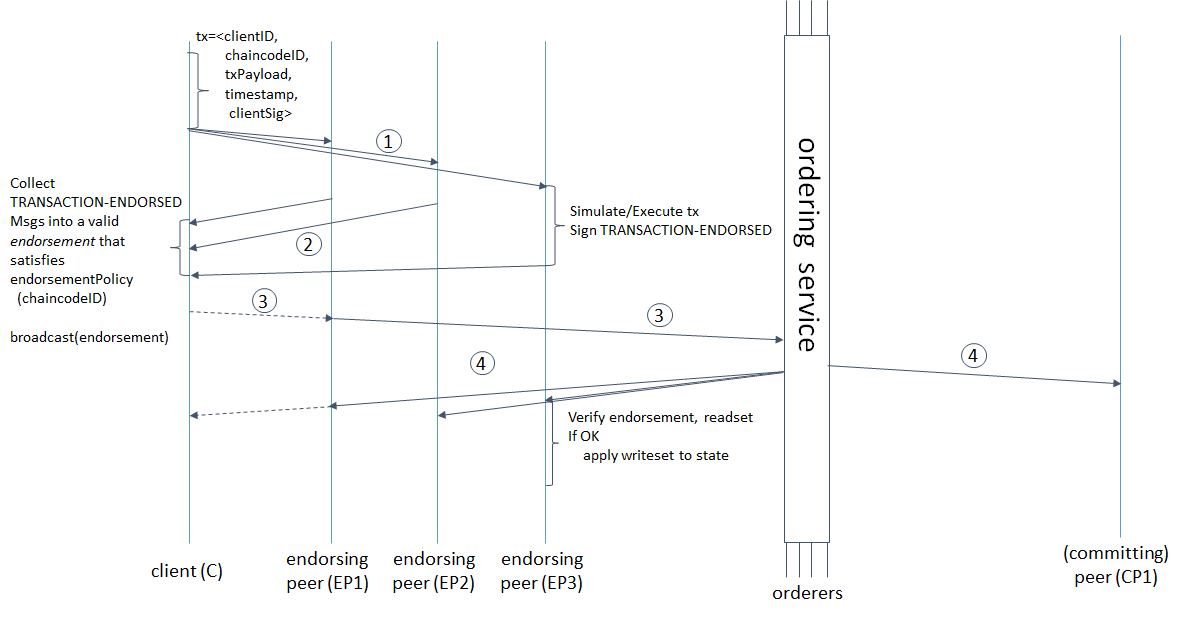
\includegraphics[width=\textwidth]{figures/fabric_transaction_flow.png}
    \end{center}
    \caption[Swimlane sequence diagram over the Hyperledger Fabric transaction flow.]{Swimlane sequence diagram over the Hyperledger Fabric transaction flow. Note that this is for an earlier version from before the Fabric gateway. As of version 2.4, the behaviour of the client in the diagram is instead performed by the gateway, while the client only initiates a transaction. The image \cite{hyperledger_transaction-flow_nodate}  was created by Hyperledger and is licensed under CC BY 4.0 \cite{noauthor_creative_nodate}.}
    \label{fig:fabric-transaction-flow}
\end{figure}

\subsection{Endorsement Policies}

An update to the Fabric ledger is only possible if the endorsement policy relevant to a transaction has been fulfilled. Endorsement policies describe which and how many organizations or peers that need to run and endorse a transaction proposal. They are defined as logical formulas referencing relevant organization and role for the peers that have to endorse it. Figure \ref{fig:endorsement-policy-example} shows an example endorsement policy with three organizations called Org1, Org2 and Org3 where all endorsing peers must have the \textit{member} role.

An endorsement policy can be defined on three different granularity levels; chaincode-, collection- and key-level. Chaincode- and collection-level policies are decided on when a chaincode is commited to the network. The former is a general policy which always has to be fulfilled everytime the chaincode submitted as a transaction. Collection-level policies on the other hand are rules for when a chaincode reads or writes from a private collection. A chaincode can have multiple private collections, each with its own collection-level policy. When a chaincode accesses such a collection, the additional policies have to be satisfied as well. Key-level policies are similar to collection-level ones in that they only become relevant when a chaincode touches a subset of the world-state. A difference being that key-level policies are declared in the execution of a chaincode. A usecase for this is when adding a new asset to the ledger with a specific owner. By setting a key-level endorsement policy to the key of the asset, any transaction that tries to change the asset will have to be endorsed by, for example, its owner before it is commited to the ledger.

\begin{figure}
    \begin{verbatim}
		OR('Org1.member', AND('Org2.member', 'Org3.member'))
	\end{verbatim}
    \caption{Endorsement policy syntax example}
    \label{fig:endorsement-policy-example}
\end{figure}

\subsection{Chaincode}

Many current blockchains have some notion of a smart contract \cite{di_pierro_what_2017}, \ie methods to programmatically change the ledger only when certain properties, or contracts, have been fulfilled. Smart contracts make blockchains more general-purpose as they can be used to model many different protocols and applications. \textbf{examples plz}

In Hyperledger Fabric, smart contracts are called chaincode. As there is no inherent asset on the Fabric ledger over which peers can make transactions, chaincodes are the only way the ledger can be changed. They are in other words the only way to create, update and remove assets. Chaincodes has to follow the \textit{fabric-contract} \gls{API} to be run by peers on the network, but what language they can be written in is flexible. The official language options are Java, Javascript and Go, but other languages can be supported in theory. Listing \ref{lst:chaincode-fabcar-example} examplifies how chaincodes can look and the mechanisms through which it interacts with the worldstate. A chaincode smart contract interacts, through the fabric-contract \glsentryshort{API}, with the world-state key-value representation of the ledger and can query, update and set values in it.

Running a chaincode on the network does not update the ledger directly (see \ref{subsec:transaction-flow} for how ledger modifications are implemented). Instead a read-write set of the keys that have been queried from and the changes to the ones that have been set during the execution of the chaincode are generated. The result of the chaincode is this read-write set, which is then further used to update the ledger itself.

\begin{listing}
    \begin{minted}[escapeinside=@@
				 , fontsize=\footnotesize
				 , tabsize=2]{JavaScript}
/*
* Copyright IBM Corp. All Rights Reserved.
*
* SPDX-License-Identifier: Apache-2.0
*/
@$\vdots$@
async queryCar(ctx, carNumber) {
	const carAsBytes = await ctx.stub.getState(carNumber);
	if (!carAsBytes || carAsBytes.length === 0) {
		throw new Error(`${carNumber} does not exist`);
	}
	return carAsBytes.toString();
}

async createCar(ctx, carNumber, make, model, color, owner) {
	const car = {
		color,
		docType: 'car',
		make,
		model,
		owner,
	};

	await ctx.stub.putState(carNumber, 
	                        Buffer.from(JSON.stringify(car)));
}

\end{minted}
    \caption{Modified chaincode excerpts from Hyperledgers sample project fabcar \cite{hyperledger_fabric-samples_2022}. The examples showcases the main chaincode API endpoints \mintinline{Javascript}{getState} and \mintinline{Javascript}{putState} for retrieving and, respectively, updating the ledger.}
    \label{lst:chaincode-fabcar-example}
\end{listing}

\todoinline{Find some good references for chaincode besides the official documentation.}

\todoinline{Describe the core api for chaincode}

\section{Formal specification}

Distributed systems can be complex to design and hard to reason about. This is mainly due to the non-deterministic interleaving of subsystems acting individually \textbf{(cite)}. To ensure that a design of a distributed system works as intended, formal specification notation and tools can be used. These do not generate actual implementations of a system, but instead a precise description of system properties \cite{lamsweerde_formal_2000}. By modeling a system with a formal specification, its properties can be automatically verified or refuted. It also forces the developer to think in terms of system invariants instead of \textit{how} the system should be constructed. Because formal specifications are models of (and not actual) systems, there is no guarantee that they correspond correctly to a real implementation. However, because they do not include as many concrete details, testing the correspondance between a specification and an implementation can be done on a higher abstraction level compared to the unit-testing common in software verification.

\todoinline{Summaries several different formal specification methods }

\section{TLA\textsuperscript+}

TLA\textsuperscript+ \cite{lamport_specifying_2001} is a language for formal specification where a model describes a systems' behaviour over time. It has been used successfully in industry to verify and finding bugs in distributed systems \cite{joshi_checking_2003,newcombe_how_2015} and can be written in both a mathematical notation style and the more pseudocode-esque PlusCal. The specification can then be verified by the TLC tool which simulates executions of the model in order to find potential faults. TLA\textsuperscript+ is built on the \gls{TLA} \cite{lamport_temporal_1994}, but adds improvements for writing more modular and larger specifications.

\subsection{\glsentryfull{TLA}}
\label{subsec:tla}

The semantics of \glsentryshort{TLA} are based on infinite sequences of states called behaviours. Here, a state $s$ is a mapping from symbolic variable names to values \eg $[x \mapsto 1, y \mapsto "a", z \mapsto 42]$. Behaviours represent the history of states that a program execution enters, one state for each atomic change. A program incrementing a counter could for example have the behaviour $\langle [x \mapsto 0, \dotsc], [x \mapsto 1, \dotsc], [x \mapsto 1, \dotsc], [x \mapsto 2, \dotsc], \dotsc \rangle$. Note that $x$ does not increment at every state in this behaviour. This is an example of \textit{stuttering} \ie $x$ is allowed to remain the same or increment at every step. Stuttering allows logical formulas, or programs, to be modular. As an example of this, we can imagine a second counter program running concurrently with the first. The two programs are both incrementing variables but not necessarily at the same time, so at certain states we need stuttering to descibe the combined program. An example of this is shown in figure \ref{fig:concurrent-behaviour}.

\begin{figure}
    $\langle [x \mapsto 0, y \mapsto 0, \dotsc], [x \mapsto 1, y \mapsto 0, \dotsc], [x \mapsto 1, y \mapsto 1, \dotsc], [x \mapsto 2, y \mapsto 2, \dotsc], \dotsc \rangle$
    \caption{A behaviour where the variables $x$ and $y$ increment concurrently.}
    \label{fig:concurrent-behaviour}
\end{figure}

\subsubsection{Propositional logic in \glsentryshort{TLA}}

The core of \glsentryshort{TLA} is propositional logic \textbf{propositional?} with common connectives \textbf{connectives?} such as $\land$, $\lor$, $\implies$, $\lnot$, $\forall$ and $\exists$.

\subsubsection{State Functions and Predicates}

\glsentryshort{TLA} allows the use of ``regular'' mathematics which can be used to form expressions such as $x^2 + 5*y - 3$. These make up the body of non-boolean state functions and their boolean equivalent predicates. The meaning of such expressions is evaluated relative a state. This is done by substituting the value of a variable in the state for the same variable in the expression. This definition can be written

\begin{math}
    s \llbracket f \rrbracket \triangleq f \lparen \forall v : s \llbracket v \rrbracket / v \rparen
\end{math}

where

\begin{itemize}
    \item $f$ is a state function or a predicate
    \item $\triangleq$ signifies equality by \textit{definition}
    \item $s \llbracket v \rrbracket$ is the value of variable $v$ in state $s$
    \item $s \llbracket v \rrbracket / v$ substitutes  $s \llbracket v \rrbracket$ for $v$
\end{itemize}

Figure \ref{fig:state-function-example} shows an example of a substitution in a state function.

\begin{figure}
    \begin{math}
        g \triangleq x + y - 2 \\
        s \triangleq \lbrack x \mapsto 0, y \mapsto 2 \rbrack \\
        s \llbracket g \rrbracket \equiv s \llbracket x \rrbracket + s \llbracket y \rrbracket - 2 \equiv 0
    \end{math}
    \caption{Semantic meaning of a state function $g$ given a state $s$.}
    \label{fig:state-function-example}
\end{figure}

\subsubsection{Actions}

So far \glsentryshort{TLA} is quite similar to propositional and predicate logic \textbf{which one?} but with the addition of \textit{actions}, it changes quite radically. An action can be seen as the link between two states in the behaviour of a program. It describes change from one state to the next. Syntactically, this is done by separating variables into two groups: \textit{un-primed} variables $x$, $y$, $z, \dotsc$ and \textit{primed} variables $x^\prime$, $y^\prime$, $z^\prime, \dotsc$. Primed variables represent the value of their un-primed counterpart in the next state, and an action is just a boolean expression with both primed and unprimed variables. Incrementing a variable can for example be written as the action $x^\prime = x + 1$. In natural language, this means that the variables value in the next state should be one more than in the previous. Similarly to how we did it for state functions and predicates, we can define the semantic meaning of an action $\mathcal{A}$ as

\begin{math}
    s \llbracket \mathcal{A} \rrbracket t \triangleq \mathcal{A}\lparen \forall v : s\llbracket v \rrbracket / v, t\llbracket v \rrbracket / v^\prime \rparen
\end{math}

where $s$ and $t$ are both states and $t$ follows directly after $s$. In other words, actions are relations between states that are following each other in time.

The changes in the increment counter program can, as mentioned, be represented by an action. To support stuttering we can add the second possibility that the variable stays the same. This is written as the disjunction $\lparen x^\prime = x + 1 \rparen \lor \lparen x^\prime = x \rparen$ \ie either $x$ is incremented or it stays the same. As it turns out, this is a commonly used concept when writing specification so \glsentryshort{TLA} provides a shorthand for it written $\lbrack \mathcal{A} \rbrack_f$. We pronounce $\lbrack \mathcal{A} \rbrack_f$ as ``square $\mathcal{A}$ sub $f$''. $f$ here is any state function, but is often a sequence of the variables that are allowed to stutter. For example, with the increment program we can write $\lbrack x^\prime = x + 1 \rbrack_{\langle x \rangle}$.

\subsubsection{Temporal operators}

Where actions describe a single step of change between two states, we have already mentioned that program executions are represented in \glsentryshort{TLA} by behaviours \ie sequences of states. To be able to describe whole behaviours we need some way of lifting actions from acting on pairs of states to sequences of states. We can perform this lifting in \glsentryshort{TLA} with the \textit{always} temporal operator, written as $\Box \mathcal{A}$. Informally, this formula is true only if the action is true for all consecutive pairs of states in a behaviour. More generally, we can write $\Box F$ where $F$ is a logical formula built from predicates and actions. For a behaviour $\langle s_0, s_1, s_2, \dotsc \rangle$, the operator can be defined as

\begin{math}
    \langle s_0, s_1, s_2, \dotsc \rangle \llbracket \Box F \rrbracket \triangleq \forall n \in \mathbb{N} : \langle s_n, s_{n+1}, s_{n+2}, \dotsc \rangle \llbracket F \rrbracket
\end{math}

where $\mathbb{N}$ is the set of natural numbers. To understand this notation, it should be noted that $\langle s_0, \dotsc \rangle \llbracket F \rrbracket$ is true if and only if $F$ is true in the behaviour's \textit{first} state $s_0$.

Besides $\Box$, another common temporal operator is called \textit{eventually} and written $\Diamond$. $\Diamond F$ denotes a formula that will be true at some point, and can be derrived in terms of the \textit{always} operator as

\begin{math}
    \Diamond F \equiv \neg \Box \neg F
\end{math}

This is equivalent to the definition

\begin{math}
    \langle s_0, s_1, s_2, \dotsc \rangle \llbracket \Diamond F \rrbracket \triangleq \exists n \in \mathbb{N} : \langle s_n, s_{n+1}, s_{n+2}, \dotsc \rangle \llbracket F \rrbracket
\end{math}

\ie $F$ should be true in \textit{some} state $s_i$. Combinations of $\Diamond$ and $\Box$ can describe some interesting properties such as

\begin{itemize}
    \item $\Box\Diamond F$, or \textit{infinietly often}
    \item $\Diamond\Box F$, or \textit{from some point onwards}
    \item $\Box \lparen F \implies \Diamond G \rparen$, or \textit{leads to}
\end{itemize}

The last one means that if $F$ is true in some state, $G$ has to be true at the same or a later state. This can also be written with the shorthand $F \leadsto G$.

\subsubsection{\glsentryshort{TLA} formulas}

Not all combinations of the above mentioned logical and temporal operators are allowed \glsentryshort{TLA} formulas. Instead, only formulas built from simple predicates (with no temporal operators or actions) or $\Box \lbrack \mathcal{A}  \rbrack_{f}$ for some action $\mathcal{A}$ and state function $f$ can be used. This is most noticable from a typical \glsentryshort{TLA} specification of a program. With an initial state predicate $init_\Phi \triangleq x = 0$ and an action describing the next state $next_\Phi \triangleq x^\prime = x + 1$, we get the \glsentryshort{TLA} formula

\begin{math}
    \Phi \triangleq init_\Phi \lor \Box \lbrack next_\Phi \rbrack_x
\end{math}

\ie either the value of $x$ is equal to 0 or it is one greater or equal to the value of $x$ in the previous state.

\subsection{TLC Model Checker}

TLA\textsuperscript+ is part of a toolbox made for supporting the creation and testing of formal specifications. Instead of validating a TLA model by hand, the TLC model checker allows mechanic verification by simulating its possible executions while looking for invalid states and other errors \cite{goos_model_1999}. If the model checker finds a problem, it terminates the simulation and notifies the user with a timeline of the behaviour that lead up to the particular error. The user can then improve their model, and gain a better understanding of their specification and system. Because verifying a specifcation means the TLC model checker has to simulate every possible behaviour, this can take a long time to do. A practical way to resolve this is to limit the state space in the model, but that also limits the type of properties that can be tested. For example, ensuring the absence of integer overflow from the sum of two 32-bit integers would imply testing all possible pairs, but this would take far too long to test. By instead limiting the possible integer values to, for example, $0 \dotsc 5$ the simulation might terminate without error but we have clearly not managed to validate the absence of overflows.

Instead, the TLC model checker is more appropriate for validating time-related and concurrency problems. An overview of some of those properties are described in the following sections.

\subsubsection*{Safety}
\label{sec:safetyProperty}

A specification that can never do anything ``bad'' is said to follow its \textit{safety} property. \textit{Bad} in this case is ambiguous but roughly means \textit{unintentional}. There are only certain states that the specification is allowed to enter without breaking its safety property. Variations of this is common to test in software engineering practices such as unit-testing. Safety checking in TLC is straightforward as it is done by simply testing every new state during simulation for the relevant property. To examplify this, we can consider type invariants as safety properties. A variable might for example only be allowed to be an integer and nothing else.

\subsubsection*{Liveness}
\label{sec:livenessProperty}

While a safe program is guaranteed to never do anything bad, whether or not it will actually do anything at all is not certain. Liveness properties describe what ``good'' things a specification necessarily will do. Some examples can be that an execution is guaranteed to terminate, that no deadlock between processes can happen, or that all processes will progress.

In TLA\textsuperscript+, liveness properties are written with temporal operators such as $\Box$ or $\Diamond$. Reaching a certain value can for example be written as $\Diamond \Box F$ \ie eventually a state is reached from which $F$ is always true.

\subsubsection*{Fairness}

Two additional examples of liveness properties are the weak and strong fairness properties. A \textit{fair} specification is guaranteed to execute an action as long as it is possible. If the action is weakly fair then it will be performed as long as it is repeatedly possible to do so. If it is strongly fair, then it will be executed unless it is no longer possible to do so at least once. More formally they are defined, for action $\mathcal{A}$ and state function $f$, as

\begin{math}
    WF_f\lparen \mathcal{A} \rparen \triangleq \lparen \Box \Diamond \langle \mathcal{A} \rangle_f \rparen \lor  \lparen \Box \Diamond \neg Enabled \langle \mathcal{A} \rangle_f \rparen \\
    SF_f\lparen \mathcal{A} \rparen \triangleq \lparen \Box \Diamond \langle \mathcal{A} \rangle_f \rparen \lor  \lparen \Diamond \Box \neg Enabled \langle \mathcal{A} \rangle_f \rparen
\end{math}

where

\begin{itemize}
    \item $\langle \mathcal{A} \rangle_f \triangleq \mathcal{A} \land \lparen f^\prime \neq f \rparen $ \ie the action $A$ is executed and changes variables in $f$
    \item $\neg Enabled \langle \mathcal{A} \rangle_f$ means that $\mathcal{A}$ is impossible to execute.
\end{itemize}


\subsection{PlusCal}

\glsentryshort{TLA} is, as can be seen in section \ref{subsec:tla}, quite different from a regular programming language. This has the benefit of being simple and flexible, but can result in hard-to-read code as specifications start to grow in size. It is also not entirely clear from its syntax how an algorithm described in for example pseudocode can be translated to it.

PlusCal is an alternative syntax specifically made for describing concurrent algorithms exactly while bringing the simplicity of writing pseudocode \cite{leucker_pluscal_2009}. It is written within a comment in a TLA\textsuperscript+ file and translated into TLA\textsuperscript+ as part of the parsing step of TLC. PlusCal is

% \subsubsection{Termination}

% \subsubsection{Deadlock}

% \subsubsection{Livelock}

% \subsection{TLA\textsuperscript+ Syntax Summary}

\section{Commitment scheme}

A commitment scheme is a cryptographic primitive for proving to a \textit{reciever} that a \textit{commiter} had some knowledge or stake at an earlier point in time without having to disclose it directly \cite{rak_automated_2017}. Given that the commiter has some public (known by both parties) value \textit{h} and stake \textit{m}, they calculate a commitment \textit{c} and an opening value \textit{d} by some method $\mathcal{C}$ \ie $\mathcal{C}(h, m) = (c, d)$. The commitment \textit{c} is sent to the reciever in this first phase of the protocol. The stake \textit{m} and the opening value \textit{d} is later sent in the second phase, from which the reciever can verify that \textit{m} was the initial value with some boolean function $\mathcal{V}(h, m, c, d)$.



% \section{Major background area 1}
% \todo[inline, backgroundcolor=kth-lightblue]{Viktigt bakgrundsområde 1}

% ...
% \subsection{\glsentryshort{WLAN} Security}% you can't use the \gls macro in a heading - but you can get the short (\glsentryshort) or long version (\glsentryshort) or \glsentrylong or even the text entry (\glsentrytext) and then there is no problem - see https://tex.stackexchange.com/questions/198140/glossaries-and-custom-section-headings-broken

\section{Related work area}
% \todo[inline, backgroundcolor=kth-lightblue]{Relaterande arbeten}

\subsection{Decentralized File Distribution}

A number of proposals for distributed and decentralized data management are recorded in the research litterature. \textcite{ince_blockchain_2020} describe a combination of blockchain and the \glsentryshort{P2P} network \gls{IPFS} for package storage. They envision a proof-of-work consensus algorithm based on the act of rebuilding a package where builders gain rewards in terms of a productiviy score with every rebuild they add to the ledger. At a certain score, a builder is promoted to an approver and can validate other builders rebuilds. Because blockchains are limited in storage space, only packages' addresses are stored in the ledger with the actual artifacts being distributed through \glsentryshort{IPFS}. While an interesting concept, no prototype or evaluation is provided by the paper. A similar approach was taken by \textcite{zichichi_efficiency_2020} but with the application of managing personal data. They managed different kinds of personal data by partitioning it through smart contracts, each with its own access list for node authorization.

Instead of using blockchain and \glsentryshort{P2P} technologies together, \textcite{blahser_thine_2021} show a prototype system for distributed package management using only a peer-to-peer technology called Hypercore protocol. They rely on Hypercore protocol to act both as a distributed file system as well as an append only ledger. This approach is convenient but does not have any built-in safeguards against malicious actors or packages. On the other hand, \textcite{liu_data_2018} used blockchain technology single-handledly to construct a distributed \gls{DNS}. Because of the limited amount of data in a zone file, no separate distributed file system was needed for their application. Each request to the service was done through a smart contract and their prototype system were able to serve requests with a 0.006025 seconds average response delay and a failure resolution rate of 2.14\%.

\subsection{Formal verification of Smart contracts}

Writing smart contracts that works correctly is hard. To aid this, several researchers have looked into using formal methods to verify them. \textcite{bhargavan_formal_2016} translated the Solidity language for writing smart contracts into the general-purpose language F$^{\star}$ made for program verification. The authors then used the type system of F$^{\star}$ to enforce certain safety properties in the smart contract. \textcite{beckert_formal_2018} took a similar approach but for the Hyperledger Fabric chaincode. By adding pre- and postconditions in comments to chaincode written in Java and translating these to Java Modeling Language \textbf{(acronym)} they managed to deduce smart contract safety properties statically. In a slightly different direction, \textcite{latif_blockchain_2019} modelled a blockchain for waste management using TLA\textsuperscript+. Their initial system description was written in UML \textbf{(acronym, cite)} which turned out to be relatively straightforward to translate into a formal specification language. The system's safety and liveness properties could then be validated with the TLC model checker.

\textcite{bracciali_building_2020} examplifies how a design-by-contract methodology \cite{meyer_applying_1992} when designing smart contracts can be enacted with TLA\textsuperscript+ modeling and verification. They specify a system for purchasing and selling estates directly in TLA\textsuperscript+ and uses its safety checks to ensure that any drawn up contract (between buyer and seller) is followed. As part of their specification, they also include checks for some vulnerabilities common in smart contracts. These include eliminating invalid and additional states and \textit{trap doors} \ie invalid events or transitions.

In  their PhD thesis, \textcite{elsayed_blockchain-based_2020} implemented a solution for trapping computer worms in a network. When a worm was detected by a host on the network, its signature was added to a blockchain built on Hyperledger Fabric. This acted as an immutable threat log, used by the network to be able to find and stop the worm. From the use of a blockchain, the log has high availability and other interesting security properties that makes it resistant to attacks. Besides implementing the system, the author moddeled with TLA\textsuperscript+ to model check its correctness, safety and liveness properties. This model included both the ineractions between smart contracts as well as the consensus algorithm used by the blockchain.

To reduce the friction between writing a veryfiable specification of a smart constract and implementing it in a regular programming language, some researchers have worked on intermediate representations from which both specifactions and implementations can be derived. \textcite{kolb_quartz_2020} describe the \textit{Quartz} language for this purpose. \textit{Quartz} is a statically typed language with which smart contracts are written as transitions in a finite-state machine. Simple authorization requirements and invariants can be annotated onto the transitions. An implementation in the Solidity smart contract language and a model in PlusCal can be derived from a \textit{Quartz} program. The finalized translation in TLA\textsuperscript+ includes a specification of the Solidity execution environment to allow a wider set of requirements to be verified while retaining ease of use. In a series of case studies they found that smart contracts written in \textit{Quartz} were on average 0.68 the number of lines of equivalent Solidity programs, while keeping execution overheads at less than $20\%$ for all cases but one.

\todoinline{Add work on infering formal specifications from logs}

% \subsection{Major related work 1}\todo[inline, backgroundcolor=kth-lightblue]{Relaterande arbeten 1}
% Carrier clouds have been suggested as a way to reduce the delay between the users and the cloud server that is providing them with content. However, there is a question of how to find the available resources in such a carrier cloud. One approach has been to disseminate resource information using an extension to OSPF-TE, see Roozbeh, Sefidcon, and Maguire \cite{roozbeh_resource_2013}.


% \subsection{Major related work}\todo[inline, backgroundcolor=kth-lightblue]{Relaterande arbeten}

% \subsection{Minor related work 1}\todo[inline, backgroundcolor=kth-lightblue]{Mindre relaterat arbete 1}


% …
% \subsection{Minor related work n}\todo[inline, backgroundcolor=kth-lightblue]{Mindre relaterat arbete n}


\section{Summary}\todo[inline, backgroundcolor=kth-lightblue]{Sammanfattning}
\todo[inline, backgroundcolor=kth-lightblue]{Det är trevligt att få detta kapitel
    avslutas med en sammanfattning. Till exempel kan du inkludera en tabell som
    sammanfattar andras idéer och fördelar och nackdelar med varje - så som
    senare kan du jämföra din lösning till var och en av dessa. Detta kommer
    också att hjälpa dig att definiera de variabler som du kommer att använda
    för din utvärdering.}

\todo[inline]{It is nice to have this chapter conclude with a summary. For
    example, you can include a table that summarizes other people's ideas and
    benefits and drawbacks with each - so as later you can compare your solution
    to each of them. This will also help you define the variables that you will
    use for your evaluation.}